\chapter{La société Capgemini}
\subsection*{Introduction}
Capgemini est une ESN\footnote{Entreprise de services du numérique} multinationale spécialisée dans le génie logiciel.
\\Elle a été créee le 1er Octobre 1967 à Grenoble par Monsieur \textsc{Serge Kampf} et elle est actuellement dirigée par  Monsieur \textsc{Paul Hermelin}.\\
En France, elle est la première dans son domaine en terme de chiffre d'affaire. \'A l'internationale, elle figure parmi les cinq premiers.
\\Capgemini est notamment côtée en bourse au CAC40.
\\\\
\begin{figure}[h]
  \captionbox{Monsieur Serge KAMPF\label{fig:dummy}}{
    
\includegraphics[width=4cm]{images/sergekampf.png}
  }
  \captionbox{Monsieur Paul HERMELIN\label{fig:dummy}}{
    
\includegraphics[width=4cm]{images/paulhermelin.png}
  }
  \captionbox{Logo de Capgemini\label{fig:dummy}}{
    
\includegraphics[width=5cm]{images/logo_capgemini.png}
  }
\end{figure}

\newpage
\section{Fiche d'identité}
\begin{description}
  \item[Raison sociale] : Capgemini
  \item[Année de création] : 1967
  \item[Fondateur] : Serge Kampf
  \item[Forme juridique] : Société anonyme à conseil d'administration
  \item[Siège social] : Paris
  \item[Directeur Général] : Paul Hermelin
  \item[Présence internationale] : 40 pays
  \item[Effectif en 2014] : 145 000
  \item[Chiffre d'affaire en 2014] : 10,6 milliards d'euros
\end{description}
\begin{figure}[h]
  \captionbox{Chiffre d'affaire par pays (2014)\label{fig:dummy}}{
    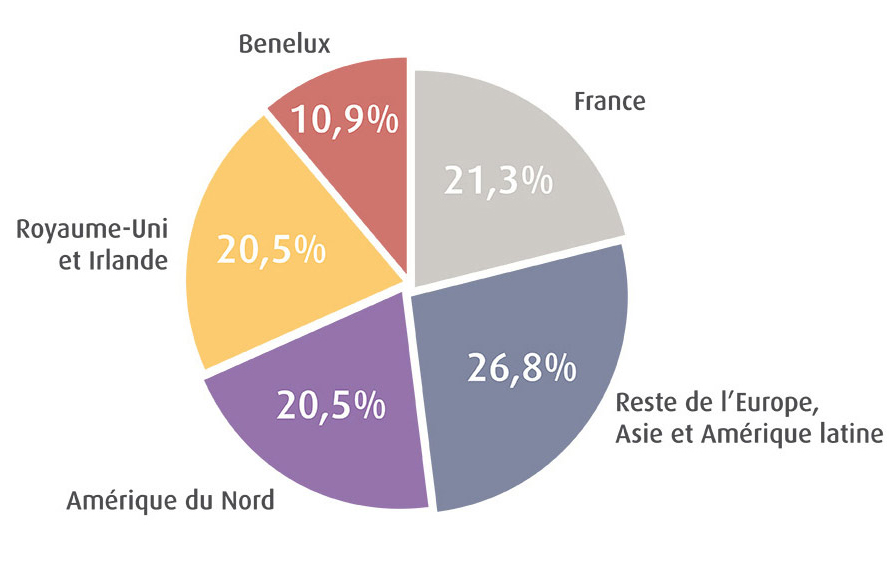
\includegraphics[width=15cm]{images/capays.png}
  }
\end{figure}
\newpage
\section{Métiers et activités}
\subsection{Secteurs d'activités}
Capgemini est spécialisé dans 6 secteurs d'activités :
\\
\begin{enumerate}
\item \textbf{Télécom, Média et \textit{Entertainment}}
\item \textbf{\'Energie, \textit{utilities} et chimie.}
\item \textbf{Industrie manufacturière et pharmaceutique}
\item \textbf{Services financiers}
\item \textbf{Grande consommation, distribution, transport et logistique}
\item \textbf{Services publics}\\
\end{enumerate}
\begin{figure}[h]
  \captionbox{Chiffre d'affaire par secteur (2014)\label{fig:dummy}}{
    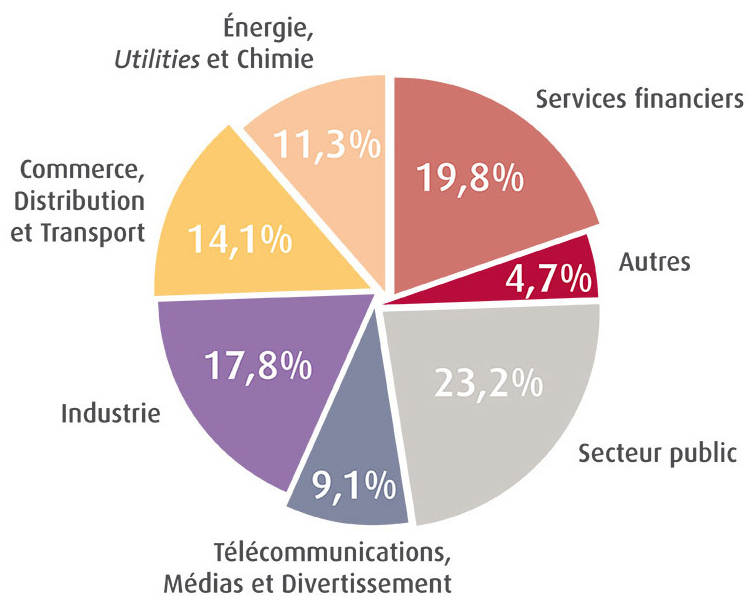
\includegraphics[width=12cm]{images/casecteur.png}
  }
\end{figure}
\newpage
\subsection{Métiers}
Capgemini travail dans 4 métiers principaux :
\\
\begin{enumerate}
\item \textbf{Le conseil en management (Capgemini Consulting)} a pour mission de contribuer, au travers d’actions telles que la transformation de l’activité ou la redéfinition de grandes fonctions, à l’amélioration des performances économiques des entreprises, grâce à une connaissance approfondie de leurs métiers et de leurs processus.
\item \textbf{L'intégration de systèmes et le développement d'applications} fait appel à la capacité de concevoir et d’intégrer des solutions, d’exploiter les innovations et de transformer l’environnement technologique.
\item \textbf{L’infogérance (Outsourcing Services - OS)} se concrétise par une prise en charge totale ou partielle de la gestion des ressources informatiques du client. Le Groupe a développé une gamme de services de gestion de systèmes informatiques, d’optimisation des processus métiers et de flexibilité des coûts de structures afin d’améliorer le rapport coût/performance.
\item \textbf{L'assistance technique et services de proximité (Sogeti)} ) sont implantés géographiquement au plus près des décideurs techniques locaux des grandes entreprises, visant à soutenir les capacités internes des directions informatiques en leur proposant dans des délais les plus brefs les meilleurs spécialistes.
\end{enumerate}
\begin{figure}[h]
  \captionbox{Chiffre d'affaire par metiers (2014)\label{fig:dummy}}{
    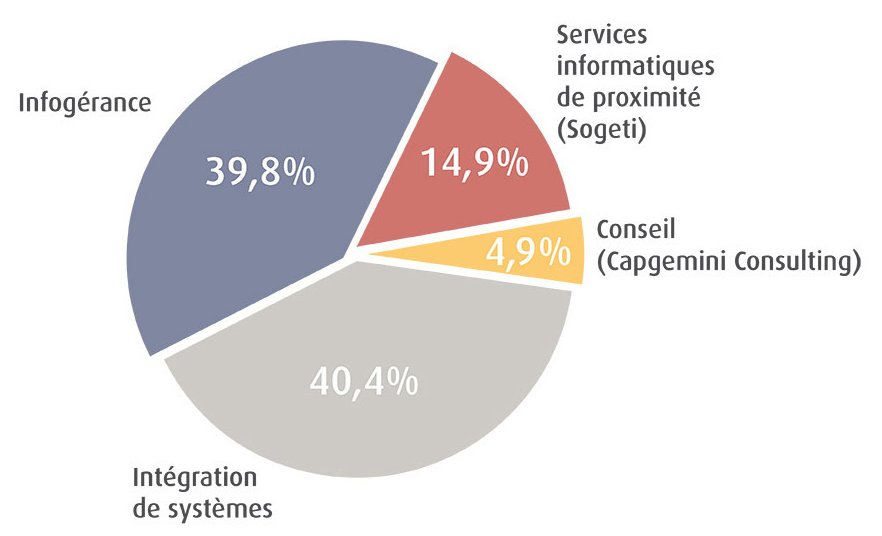
\includegraphics[width=13cm]{images/cametier.png}
  }
\end{figure}
